\section{Results}

Here we discuss the generation and analysis of the initial replicate runs, followed by the more detailed results from each of the four case study lineages.

\begin{figure}[!h]
\begin{center}
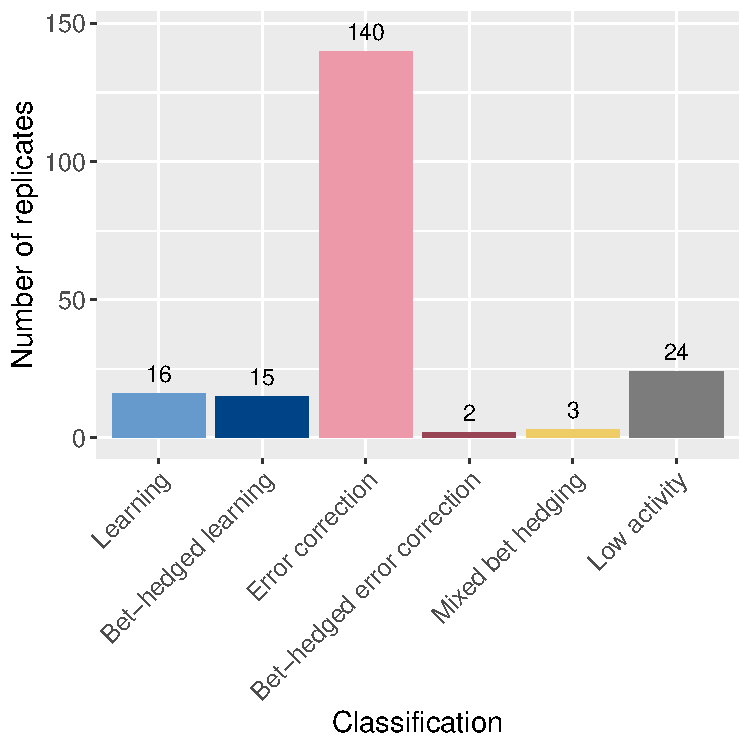
\includegraphics[width=0.45\textwidth]{02_alife_2023_submission/media/final_dom_classification.pdf}
\caption{Behavior classification of the final dominant genotypes from the 200 initial parallel replicates.}
\label{fig-final-dom-classification}
\end{center}
\end{figure}

% \begin{figure}[t]
% \begin{center}
% 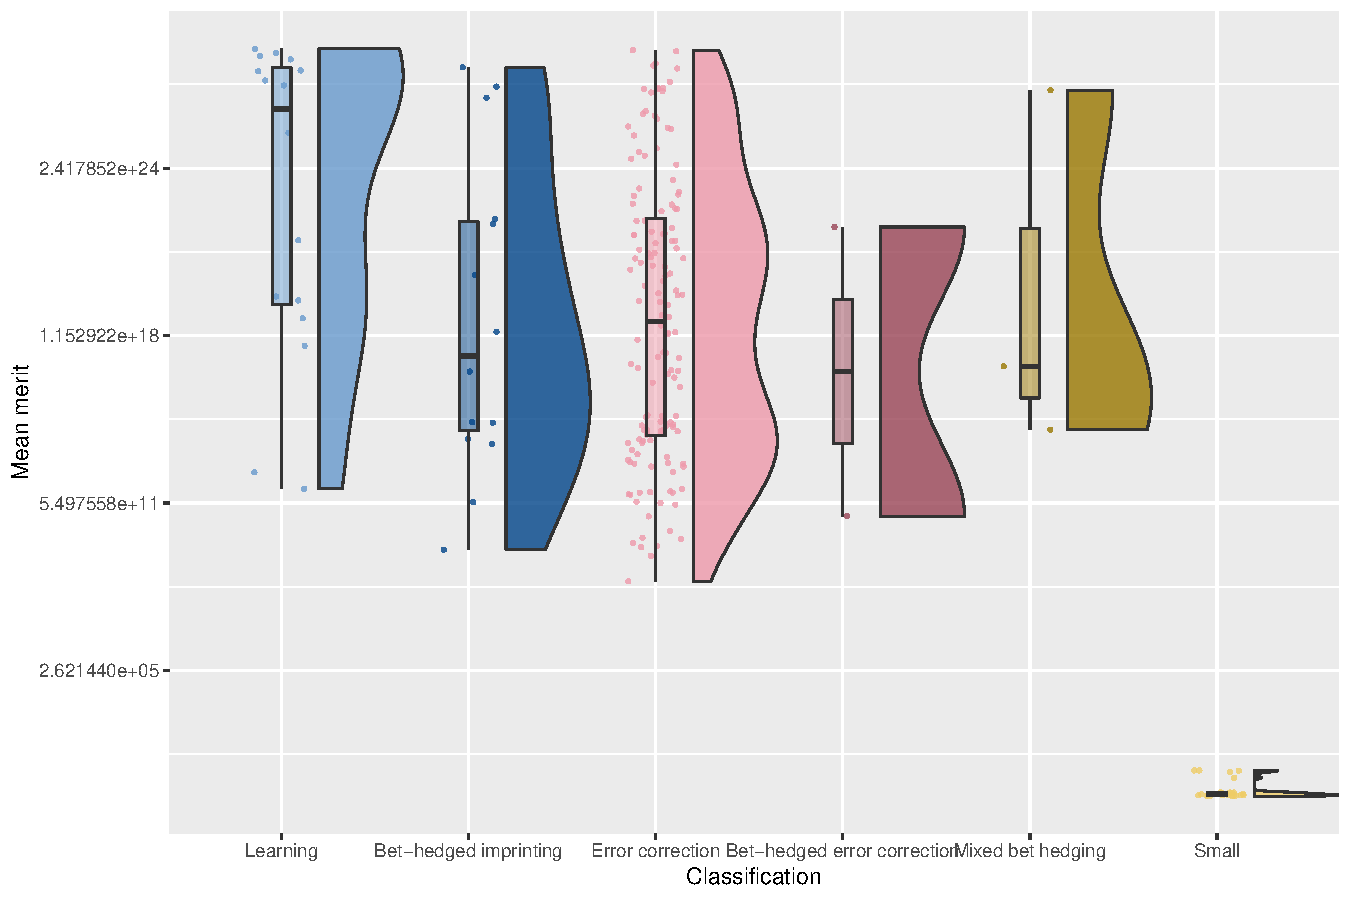
\includegraphics[width=0.45\textwidth]{media/raincloud_rep_merit.pdf}
% \caption{TODO}
% \label{fig-final-dom-rep-merit}
% \end{center}
% \end{figure}

\subsection{Evolution of learning in the initial replicates}
In the first phase of this study, we evolved 200 independent replicates for 250,000 updates (about 3600 generations) in the associative learning domain, each starting with a default ancestor.% capable only of self-replication.
%This setup allowed populations to experience approximately 3600 generations; 
The distribution of evolved behaviors is shown in Figure \ref{fig-final-dom-classification}.
Only 16 of 200 replicates exhibited associative learning.
An additional 15 replicates evolved forms of bet-hedged learning, with two of those replicates gaining and then losing associative learning along their lineage.
The majority of replicates relied on some form of error correction, either as a sole strategy (140), a bet-hedged variant (2), or as a fallback due to limited learning (3). 
%Both bet-hedged error correction replicates have a subset of environments that caused them to fall into cycles of repeatedly choosing the wrong action.%choosing the wrong action, backing up, and then choosing the same wrong action. 
%This prevented them from gaining any additional fitness. 
%Of the three mixed bet-hedging replicates, one exhibited learning in one environment and error correction in the other three
%The other two replicates exhibited the same behavior in all environments: a pseudo-learning strategy that failed on certain sequences of cues and fell back on error correction too often to hit the 90\% accuracy required to be classified as learning.
Finally, 24 replicates failed to navigate enough states to categorize them, leading us to label them as ``low activity''. 

We analyzed all 16 replicates that evolved and maintained learning, identifying the length of their lineages from onset of evolution until learning stabilized, no longer showing further improvement.
Given the substantial computational power required for each time point studied, we performed replay experiments only on the shortest three such lineages (lineages A-C), plus the shortest lineage that exhibited error correction at some point in its evolutionary history (lineage D).
%Of the 16 replicates that evolved and maintained learning, we performed replay experiments on four of them.
%The first three replicates were selected for having the shortest number of steps along a lineage before fitness stopped increasing. 
%The fourth was selected for the same reason, but was selected from among the four replicates that contained error correction in their lineages. 
%These replicates were selected to save computational resources.
%The number of updates experienced by a replay replicate was calculated as the number of updates between the genotype's first appearance in the population and the 250,000 update limit for the initial replicates. 
%Thus longer lineages A) have the potential to require more exploratory replays before saturating to $>90$\% potentiation and B) typically require more updates per replay for early steps in the lineage. 
Selecting these particular replicates to replay has the potential to bias the results, as discussed below.

% \begin{table}[!t]
% \centering
%     {\rowcolors{2}{white}{lightgray!20}
%     \begin{tabular}{ |c|c|c|c|c| }
%         \hline
% %        \makecell{Lineage} & \makecell{Initial \\ seed} & \makecell{Potentiating \\ mutation depth} & \makecell{Potentiation \\ increase} & \makecell{Fitness \\ effect} &  \makecell{Steps before \\ learning} & \makecell{Percentage of \\ updates persisted} \\
%         % \makecell{Lineage} & \makecell{Initial \\ seed} & \makecell{Potentiating \\ mutation depth} & \makecell{Potentiation \\ increase} & \makecell{Fitness \\ effect} &  \makecell{Steps before \\ learning} & \makecell{Potentiating \\ mutation persistence} \\
%         % \hline
%         % A & 86 & 484 & 58pp & Neutral & 53 & 89\% \\ 
%         % B & 4 & 104 & 36pp & Beneficial & 91 & 100\% \\ %1096 (all) \\ 
%         % C & 15 & 279 & 64pp & Deleterious & 26 & 100\% \\ %1978 (all) \\ 
%         % D & 6 & 548 & 50pp & Neutral & 8 & 100\% \\ %589 (all) \\ 
%         \makecell{Lineage} & \makecell{ mutation \\ depth} & \makecell{Potent. \\ increase} & \makecell{Fitness \\ effect} &  \makecell{Steps to \\ learning} \\
%         \hline
%         A & 484 & 58pp & Neutral & 53 \\ 
%         B & 104 & 36pp & $+$ & 91 \\ %1096 (all) \\ 
%         C & 279 & 64pp & $-$ & 26 \\ %1978 (all) \\ 
%         D & 548 & 50pp & Neutral & 8 \\ %589 (all) \\ 

%         \hline
%     \end{tabular}
%     \caption{
%     Summary of targeted replay traits.
%     }
%     \label{tab:replay-summary}
%     }
% \end{table}

\subsection{Case studies of individual lineages}

\begin{figure*}[!th]
    \begin{center}
    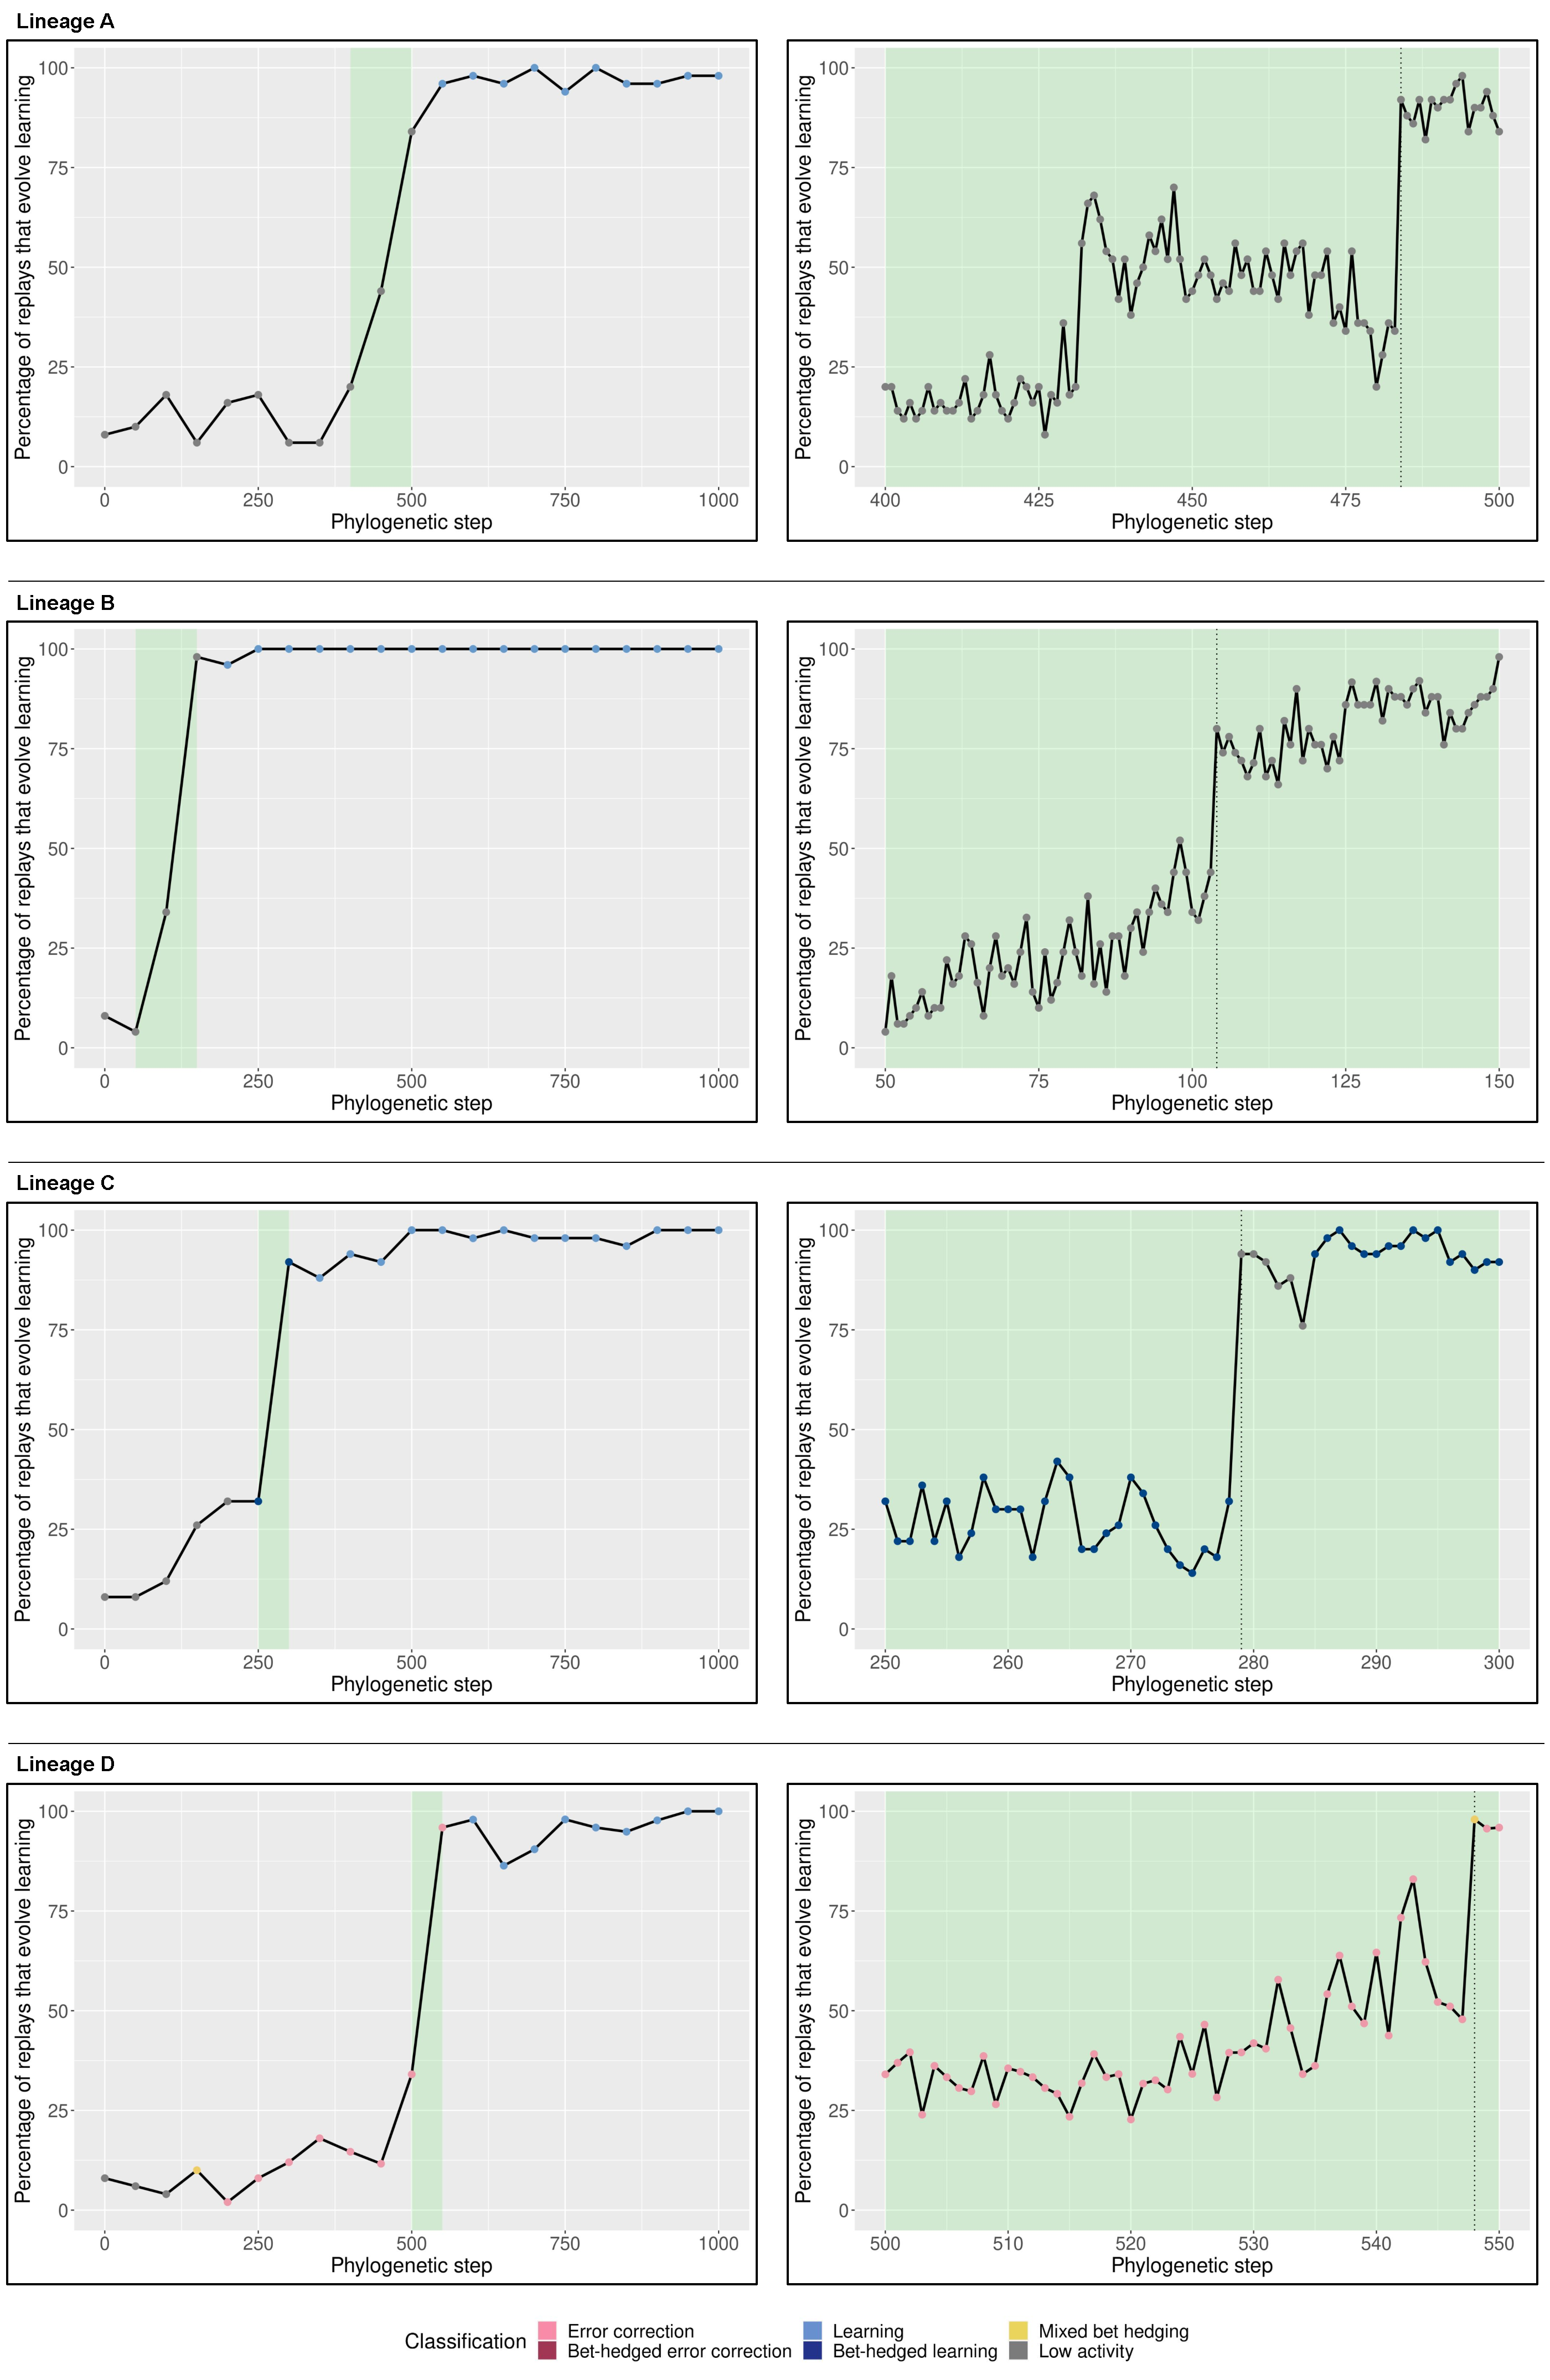
\includegraphics[width=0.72\textwidth]{02_alife_2023_submission/media/combined_replay_plots.pdf}
    \caption{
        Potentiation of associative learning for all case studies, shown as the percentage of replicates that evolve associative learning when evolution is replayed starting at that point.%, as it changes over the lineage for the four case studies. 
        For each case study, the left plot shows the results of the exploratory replays. 
        We identified a window of increased potentiation in each lineage, indicated by the shaded region. 
        Within that window, we conducted targeted replays for every step along the lineage. 
        The results of those targeted replays are shown in the plots on the right.
        The color of the points corresponds to the behavior exhibited at that step of the lineage. 
        A dotted line in the targeted replays indicates the mutation that confers the most potentiation.
    }
    \label{fig-potentiation-all-case-studies}
    \end{center}
\end{figure*}

Below we present the results of the replay experiments performed on the four focal lineages and provide a step-by-step analysis of how key mutations altered both immediate fitness and evolutionary potential (potentiation).
Where possible, we explained how these mutations altered the underlying algorithms.
For each lineage, potentiation across both exploratory and targeted replays can be found in Figure \ref{fig-potentiation-all-case-studies}.
%Additionally, details about the most-potentiating mutation from each lineage can be found in Table \ref{tab:replay-summary}.

\subsubsection{Lineage A}

% \begin{figure}[!h]
%     \begin{center}
%     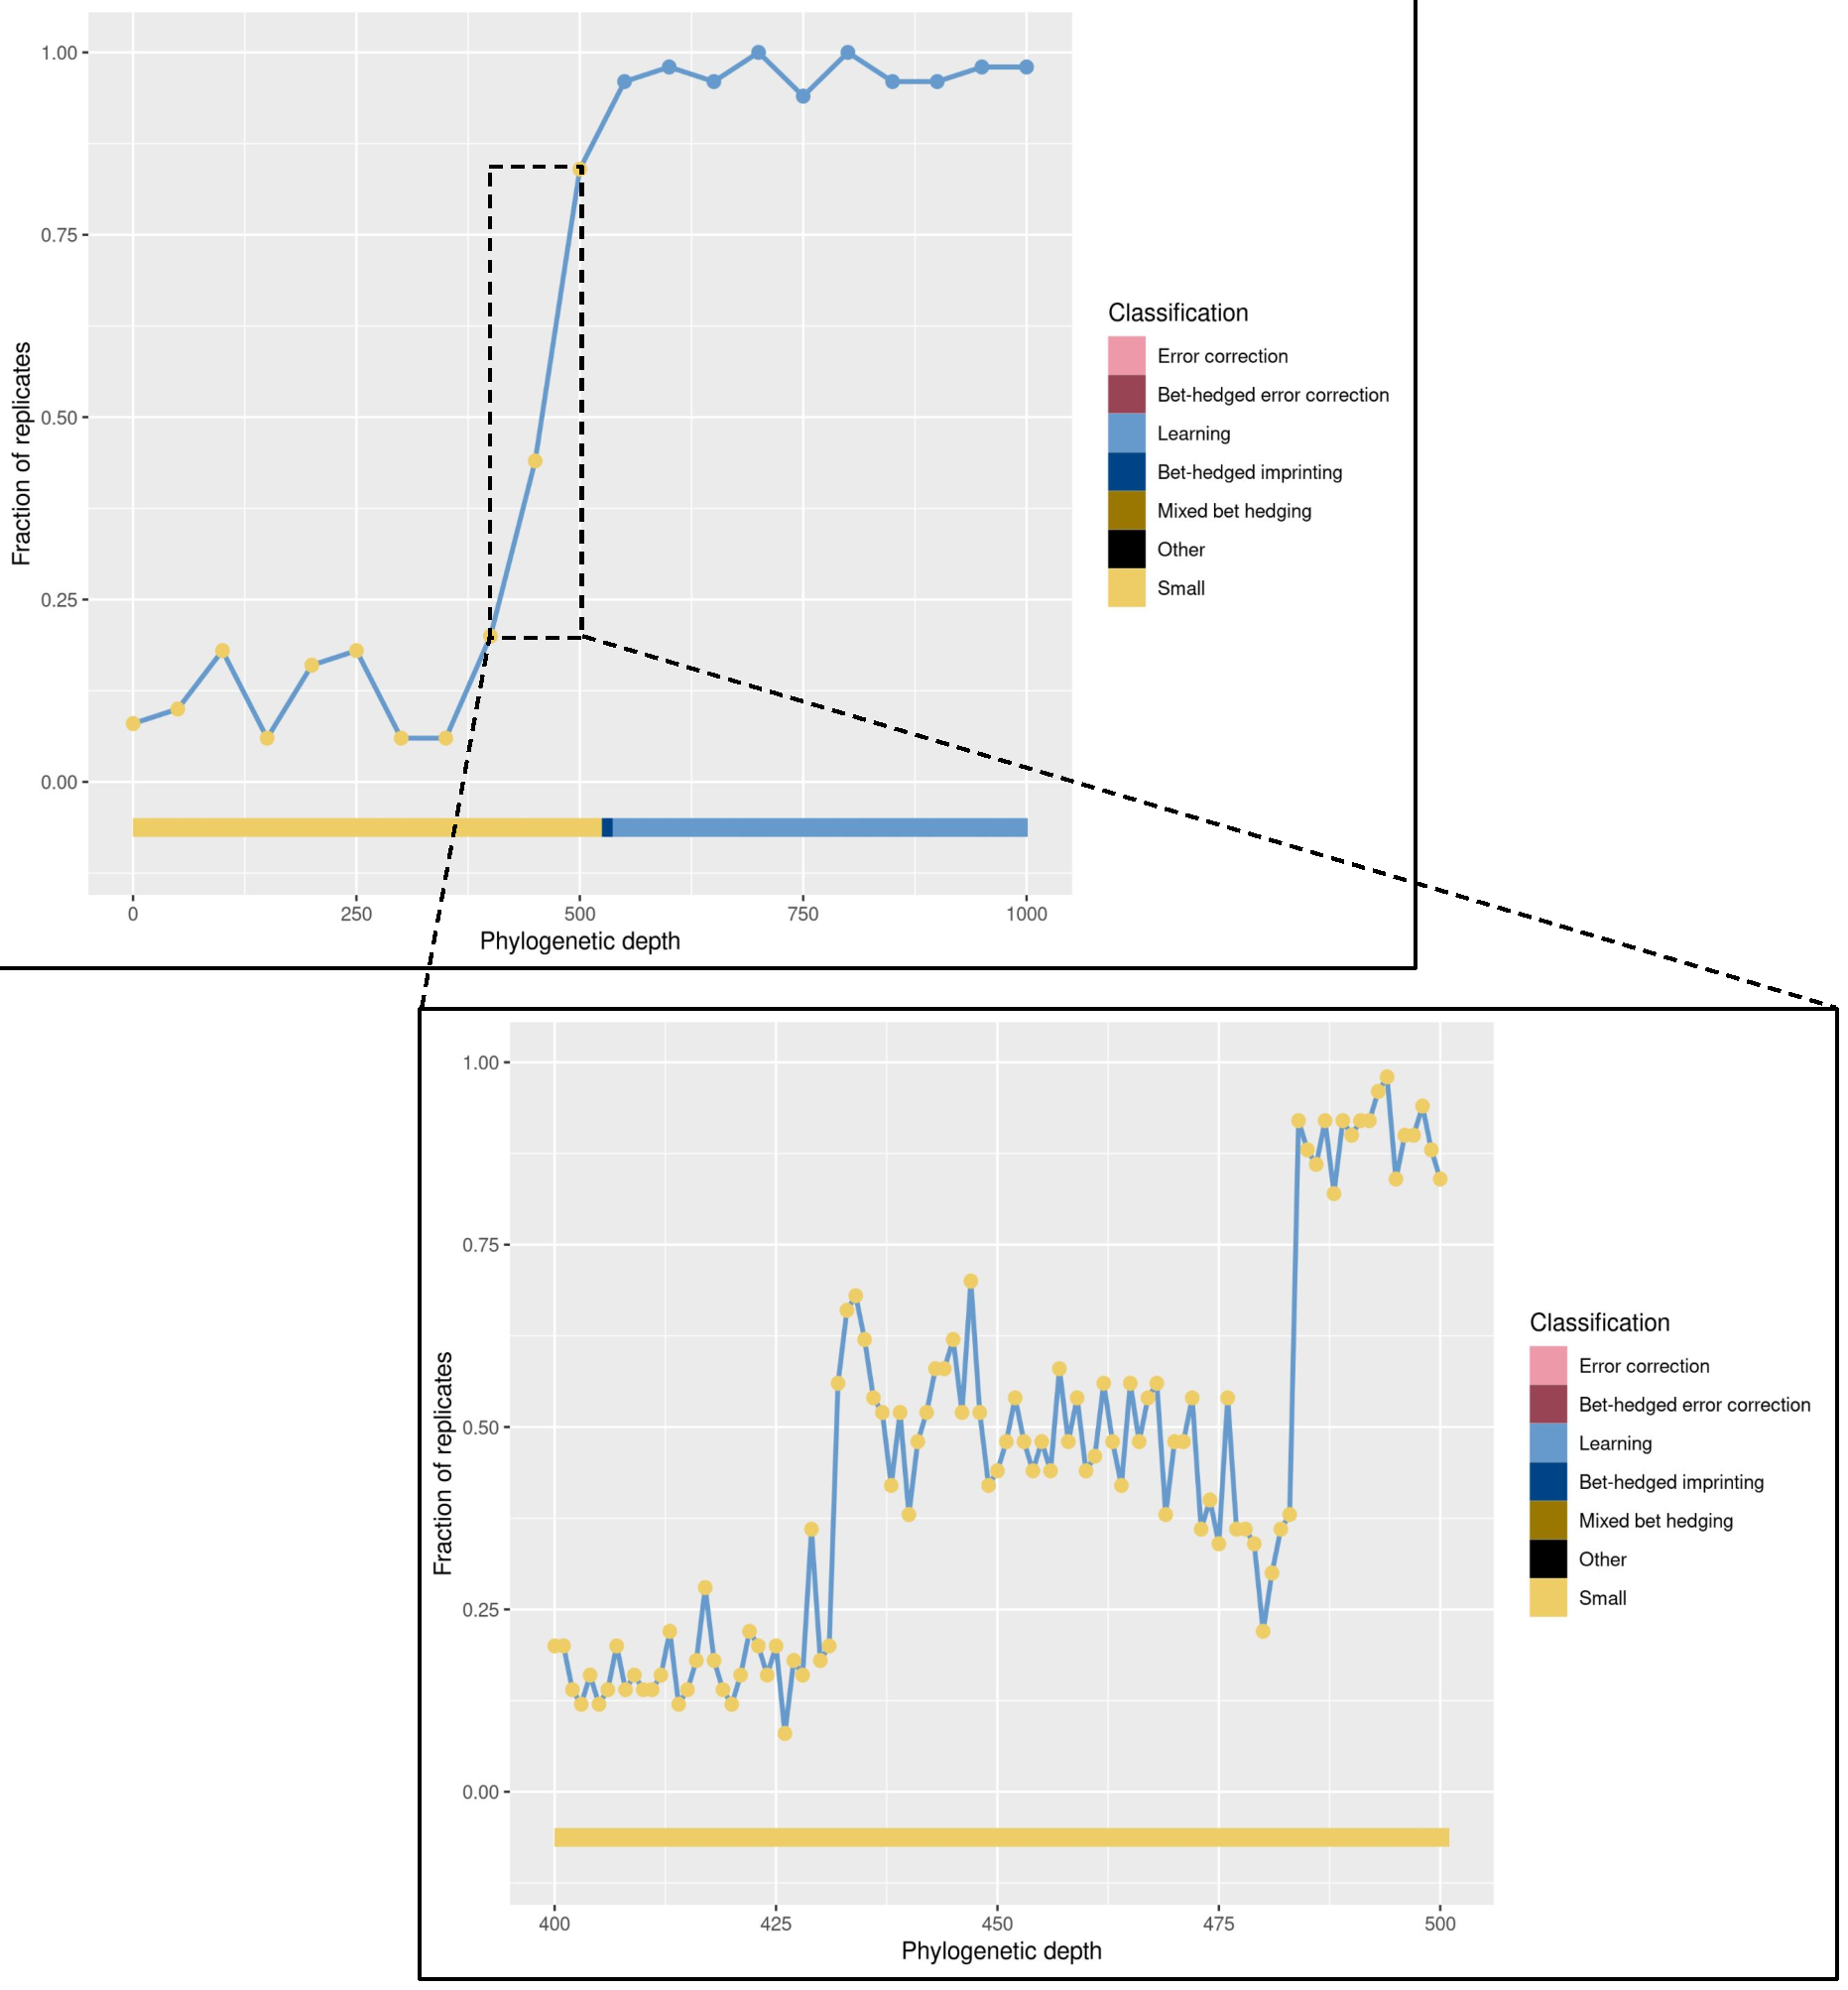
\includegraphics[width=0.45\textwidth]{media/test_pop_out_seed_86.pdf}
%     \caption{
%         \textbf{Case Study A}.
%         Potentiation of associative learning, shown as the fraction of replicates that evolve associative learning when replays are started at that point, as it changes over the lineage for Case Study A. 
%         The top figure plot shows the results of the exploratory replays. 
%         Two windows of increased potentiation were identified, indicated by the dashed rectangle. 
%         Results of the targeted replays are shown in the bottom, pop-out plot.
%         Both lines and points show potentiation at various steps along the lineage. 
%         The color of the points corresponds to the behavior exhibited at that step of the lineage.
%         The rectangle at the bottom of the plot also shows the behavior at the lineage, but with more detail than the evenly spaced points of the exploratory replay.
%     }
%     \label{fig-potentiation-case-study-a}
%     \end{center}
% \end{figure}

Our first case study is one of the shortest lineages and it contains a quick jump to learning (at step 537) from low activity, with only a brief time spent in bet-hedged learning. 
%The exploratory and targeted replays for Case Study A are both shown in Figure \ref{fig-potentiation-case-study-a}.
Exploratory replays for this lineage revealed a stark jump in potentiation between 400 and 500 steps from the ancestor, which we call the potentiation window.
From step 400 to step 450, potentiation increased from 20\% of replicates to 44\%, and increased again to 84\% of replicates by step 500. 
Before this window, potentiation fluctuated around the original 8\% found starting from the default ancestor.
%Before this jump, the potentiation fluctuates between 6\% of replicates and 20\% of replicates evolving learning. 
After the selected window, potentiation increased once more and then fluctuated between 94\% and 100\%. 

With this in mind, we seeded 50 replays for each genotype in the potentiation window. 
%Since we run 50 replicates at each step, there is considerable noise in the data. 
%Regardless, two mutations confer drastic increases in potentiation: steps 432 and 484. 
Even with the noise due to a small sample size, %that comes from having only 50 replays at each step,
we identified two mutations that conferred sizable increases in potentiation: steps 432 and 484.
The mutation at step 432 brought potentiation above 50\% for the first observed time in the lineage. 
Surprisingly, potentiation then decreased (on average) back to a local minimum of 20\% of replicates at step 480. 
Finally, the mutation at step 484 substantially increased potentiation to 92\%, where it stayed for all subsequent replays. 
%Looking at performance averaged over 100 trials, both mutations are neutral in fitness.

Even though the largest jump in potentiation occurred at step 484, learning did not appear in the lineage until step 537. 
That said, only steps 516 and 525 caused any change in behavior; all other interim mutations occurred in unexecuted regions of the genome. 
The potentiating mutation at step 484 made a key instruction in the main loop of the genome redundant.
It had no immediate effect on fitness, but later (in intermediate step 516) allowed the redundant instruction to be replaced by
%, mutating the redundant instruction into 
a right turn that granted a small fitness increase as organisms could now navigate until they reached the second left turn. 
Step 525 further improved navigation, but used a comparison that made an unfounded assumption on whether the left or right random cue is larger. 
When the assumption was correct organisms were capable of learning the cues, however the assumption is only correct 50\% of the time, so this genotype is categorized as bet-hedged learning. 
Finally, step 537 swapped that comparison with one that makes no assumptions about cue values, enabling the genotype to learn in all environments.%and now the genotype can always learn. 

Looking at the local mutational neighborhood, the potentiating mutation at step 484 increased the number of two-step mutations that conferred learning from 2 to 9 (of approximately 56 million). 
Additionally, the fitness of the learning mutations in the local neighborhood increased by three or four orders of magnitude.
%Specifically, the mutation at step 484 adds a \texttt{Decrement} instruction at the very first position in the genome. 
%This makes another \texttt{Decrement} instruction in the midst of the main section of the genome obsolete, as it was only called once and now is never called because of the new mutation. 
%With that locus now free to mutate, step 516 sees a mutation at that exact locus, swapping it to a \texttt{Right} movement instruction.
%This allows organisms to move right for the first time, which they do successfully a few times before being stumped by a \textit{left} immediately followed by a \textit{right}.
%Finally, the mutation to learning at step 537 adds more flow control before the new \texttt{Right} instruction, alleviating the issue and allowing organisms to cleanly handle any sequence of states. 
%These three mutations saw a shift from less than 7 correct states, on average, at step 484, to less than 10 at step 516, to over 115 at step 537, resulting in a drastic fitness increase.
%While was purely neutral in fitness when it occurred, the mutation at step 484 shifted the genetic material to allow changes to the vital machinery and paving the way for learning. 

What about the earlier potentiation that was gained and then lost?
The mutation that substantially increased potentiation at step 432  introduced a comparison that had no immediate fitness effect. 
This comparison remained unimportant until step 525 when it became integral in introducing bet-hedged learning.%interacted with that new comparison to improve the algorithm. 
%Looking at two-step mutations, neither step 432 nor the step before had any learning in their local landscapes. 
Neither step 432 nor its predecessor had access to learning within a two-step mutational range.
Thus, it is likely that the potentiation comes from that comparison given that we observed it being utilized for learning later on.

%The earlier potentiation at step 432 swapped a \texttt{Push} instruction for an \texttt{IfLess} instruction. 
%At the time, this did nothing. 
%In fact, this instruction only comes into play at step 537, where it becomes part of the logic of ``if B does not equal C AND C is greater than or equal to 3, then take a right turn''. 
%Thus, while it took a while to get there, the mutation was directly useful in the learning algorithm. 

%[MOVE TO DISCUSSION???]
Why then, did potentiation decrease between steps 432 and 484?
At step 432 (and indeed before it), the algorithm had a section where if register B was non-zero, then B stored the cue associated with a left turn. 
While this information was likely to make the evolution of learning easier, it was unused at that time. 
As such, the mutations between steps 432 and 484 dismantled that machinery, requiring a replacement to be built before learning could evolve.

%increasing the number of mutations needed for learning to evolve. 
%Indeed, this machinery was rebuilt before learning evolved, but in a different way. 

\subsubsection{Lineage B}

% \begin{figure}[!h]
% \begin{center}
% 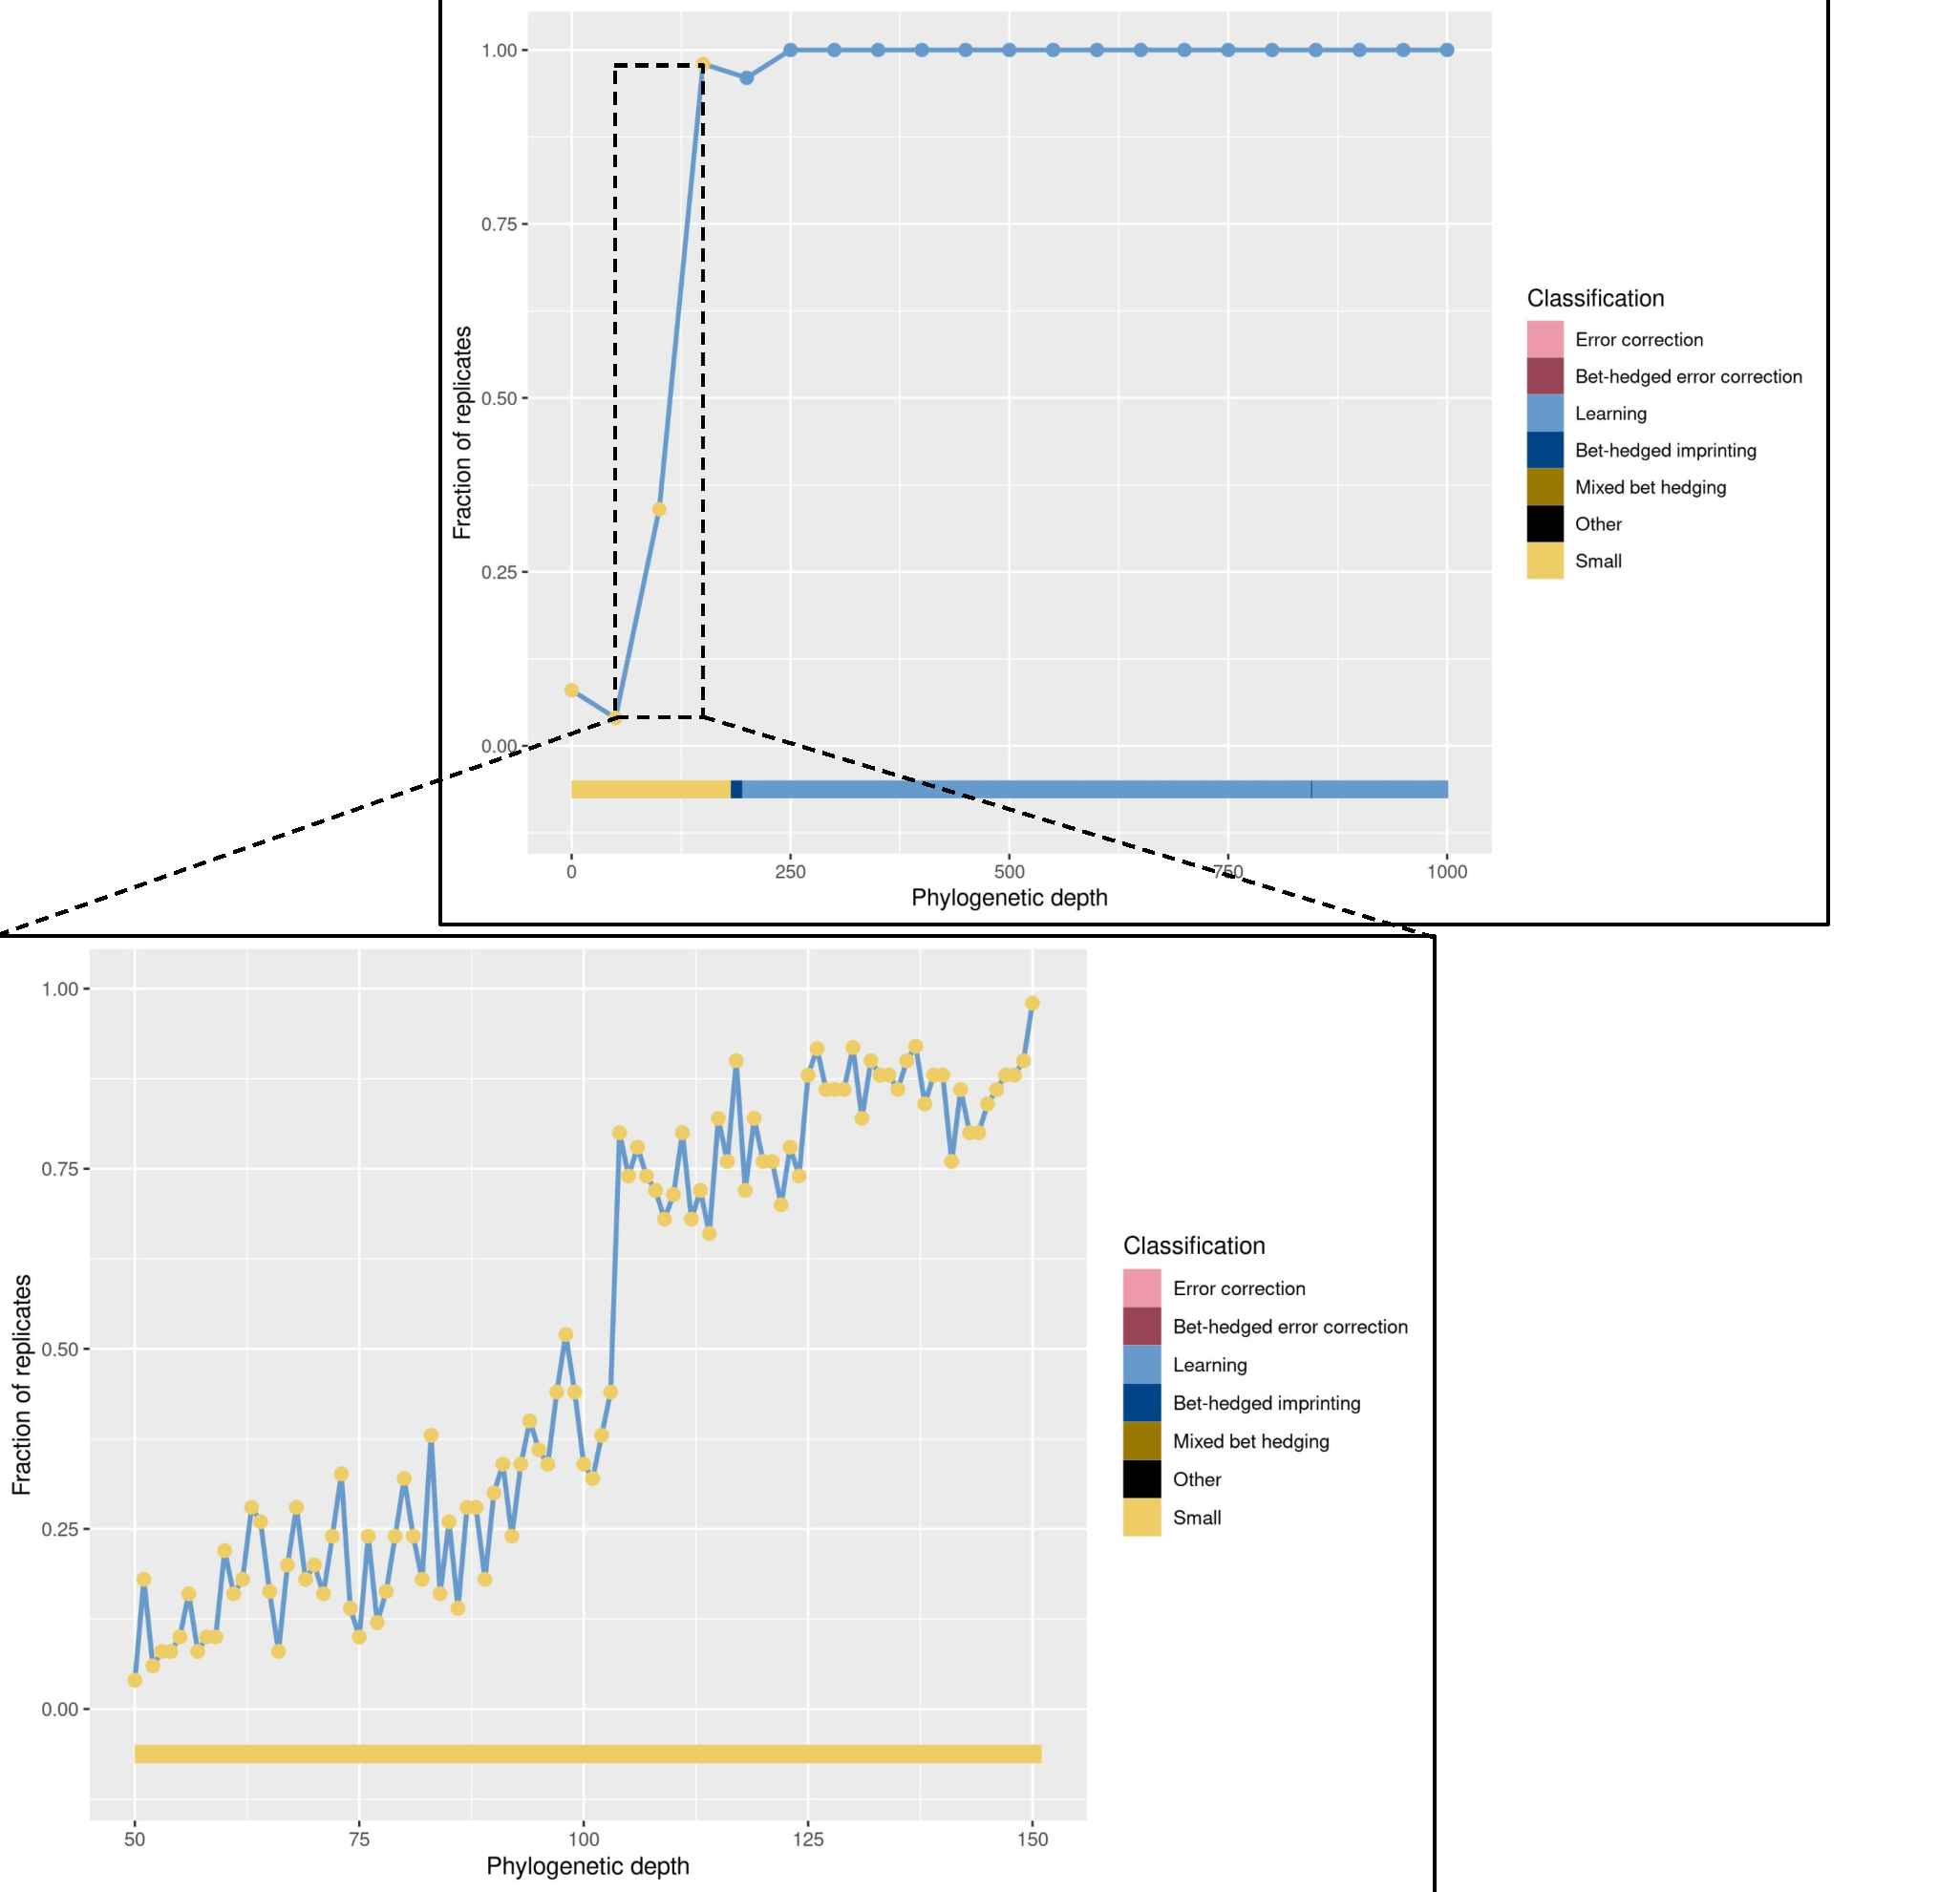
\includegraphics[width=0.45\textwidth]{media/test_pop_out_seed_4.pdf}
% \caption{
% \textbf{Case Study B}.
% Potentiation of associative learning as it changes over the lineage for Case Study B. 
% The top figure plot shows the results of the exploratory replays. 
% Two windows of increased potentiation were identified, indicated by the dashed rectangle. 
% Results of the targeted replays are shown in the bottom, pop-out plot.
% Both lines and points show potentiation at various steps along the lineage. 
% The color of the points corresponds to the behavior exhibited at that step of the lineage.
% The rectangle at the bottom of the plot also shows the behavior at the lineage, but with more detail than the evenly spaced points of the exploratory replay.}
% \label{fig-potentiation-case-study-b}
% \end{center}
% \end{figure}

Similar to Lineage A, this lineage transitioned from low activity to learning through a brief period of bet-hedged learning. 
Exploratory replays on this lineage reveal that learning was potentiated almost immediately; by step 150 potentiation had climbed above 95\%, where it stayed for the rest of the lineage. 
%From this exploration we identified 
As such, the potentiation window included steps 50 through 150.%, and therefore targeted that windows for additional replays. 

Unlike Lineage A, the targeted replays reveal a general trend of increasing potentiation, with step 104 as a notable outlier. 
%However, one mutation stands out as an outlier: step 104. 
Mutations from steps 50 through 103 slowly increased potentiation from 4\% to 44\%, but the mutation at step 104 jumped it to 80\%. 
From there, another slow increase continued to raise potentiation to a peak of 98\% at step 150.

Learning did not appear until step 195, over 90 steps beyond the largest potentiating mutation. 
Given that 34 interacting mutations altered the encoded algorithm, the mechanistic pathway to achieve learning is more complicated than can be broken down in this work.
%breaking down the exact details of the changes to reach learning is beyond the scope of this work. 
However, the potentiating mutation at step 104 modified the execution flow of the genome, which appears to have been later used essential for the later evolution of learning.% in the long term. 

While two mutations occurred at step 104, only one caused a functional change: an instruction to swap data between registers was mutated to a left turn. 
Prior to this mutation, the genome encoded a left turn later on, after which the execution became trapped in an endless loop. 
The potentiating mutation was immediately beneficial; it allowed organisms to take the left turn earlier, which, in turn, allowed them to avoid the loop. 
%As such, this mutation was immediately beneficial when it occurred. 
In avoiding the infinite loop, a large portion of the genome was now skipped and remained so when learning evolved 91 steps later. 
Looking at the local fitness landscape, learning was neither present in the potentiating step's landscape nor in the step before.
We hypothesize that the potentiation came from the change in structure of the genome, that skipping the execution of those instructions avoided a pitfall and freed up execution time that may have been useful in evolving learning.

%While two mutations occurred at step 104, only one provides a functional change. 
%That mutation is a point mutation swapping a \texttt{Swap} instruction for a \texttt{Left} movement instruction. 
%Another \texttt{Left} instruction already existed a little further along the genome, but removing the \texttt{Swap} instruction allowed execution to jump back to the main portion of the genome, while still executing the needed left turn before doing so. 
%This increased fitness immediately, as it prevented the organism from getting stuck in an infinite loop at toward the end of the genome, instead correctly handling a few more states. 
%Secondly, this caused a large portion of the genome to not be executed, most of which is still skipped when learning evolved at step 195. 
%The mutation at step 104 did prove important, as it persisted throughout evolution, being present in the final genome at step 1544.


\subsubsection{Lineage C}

Lineage C has the biggest single-mutation potentiation increase (64 percentage points), and that mutation was deleterious when it occurred at step 279 along the lineage.  Learning later appeared at step 305. 

The potentiating step mutated a no-operation instruction into a conditional flow control instruction. 
%On the existing genetic background, this mutation was terrible for fitness.
At step 278 the genotype was capable of bet-hedged learning, but the mutation at 279 knocked out all instances of learning, reclassifying the lineage as ``low activity.'' %down below the classification threshold. 
The next step restored some fitness, and then step 285 interacted with the mutation at 279 to not only restore fitness, but to dramatically improve it. 
Ultimately, the potentiating mutation allowed the algorithm to more precisely discriminate between the left and right cues. 
Prior to the mutation, it used a less-than comparison, which only functioned correctly in tests where the ``turn left'' cue was less than the ``turn right'' cue. %left the algorithm at the mercy of the random cue values. 
The potentiating mutation switched it to an equality comparison, which alleviated the assumption that one cue will be larger than the other.

Interestingly, the potentiating mutation both lowered the number of learning mutations available in the local fitness landscape and decreased the average fitness of the learning mutants that do exist. 


% When learning appears at step 305, it comes in the form of a \texttt{Decrement} instruction being swapped for a \texttt{Subtract}.
% These genotypes cannot fix their mistakes, they rely on never making errors. 
% Steps 285 through 304 cannot handle two \textit{left} states in a row, but step 305 can. 
% By using subtraction instead of decrement, the algorithm is able to always zero out the register, which combines with the flow control and ensures the algorithm can handle multiple left turns in a row.



% \begin{figure}[!h]
% \begin{center}
% 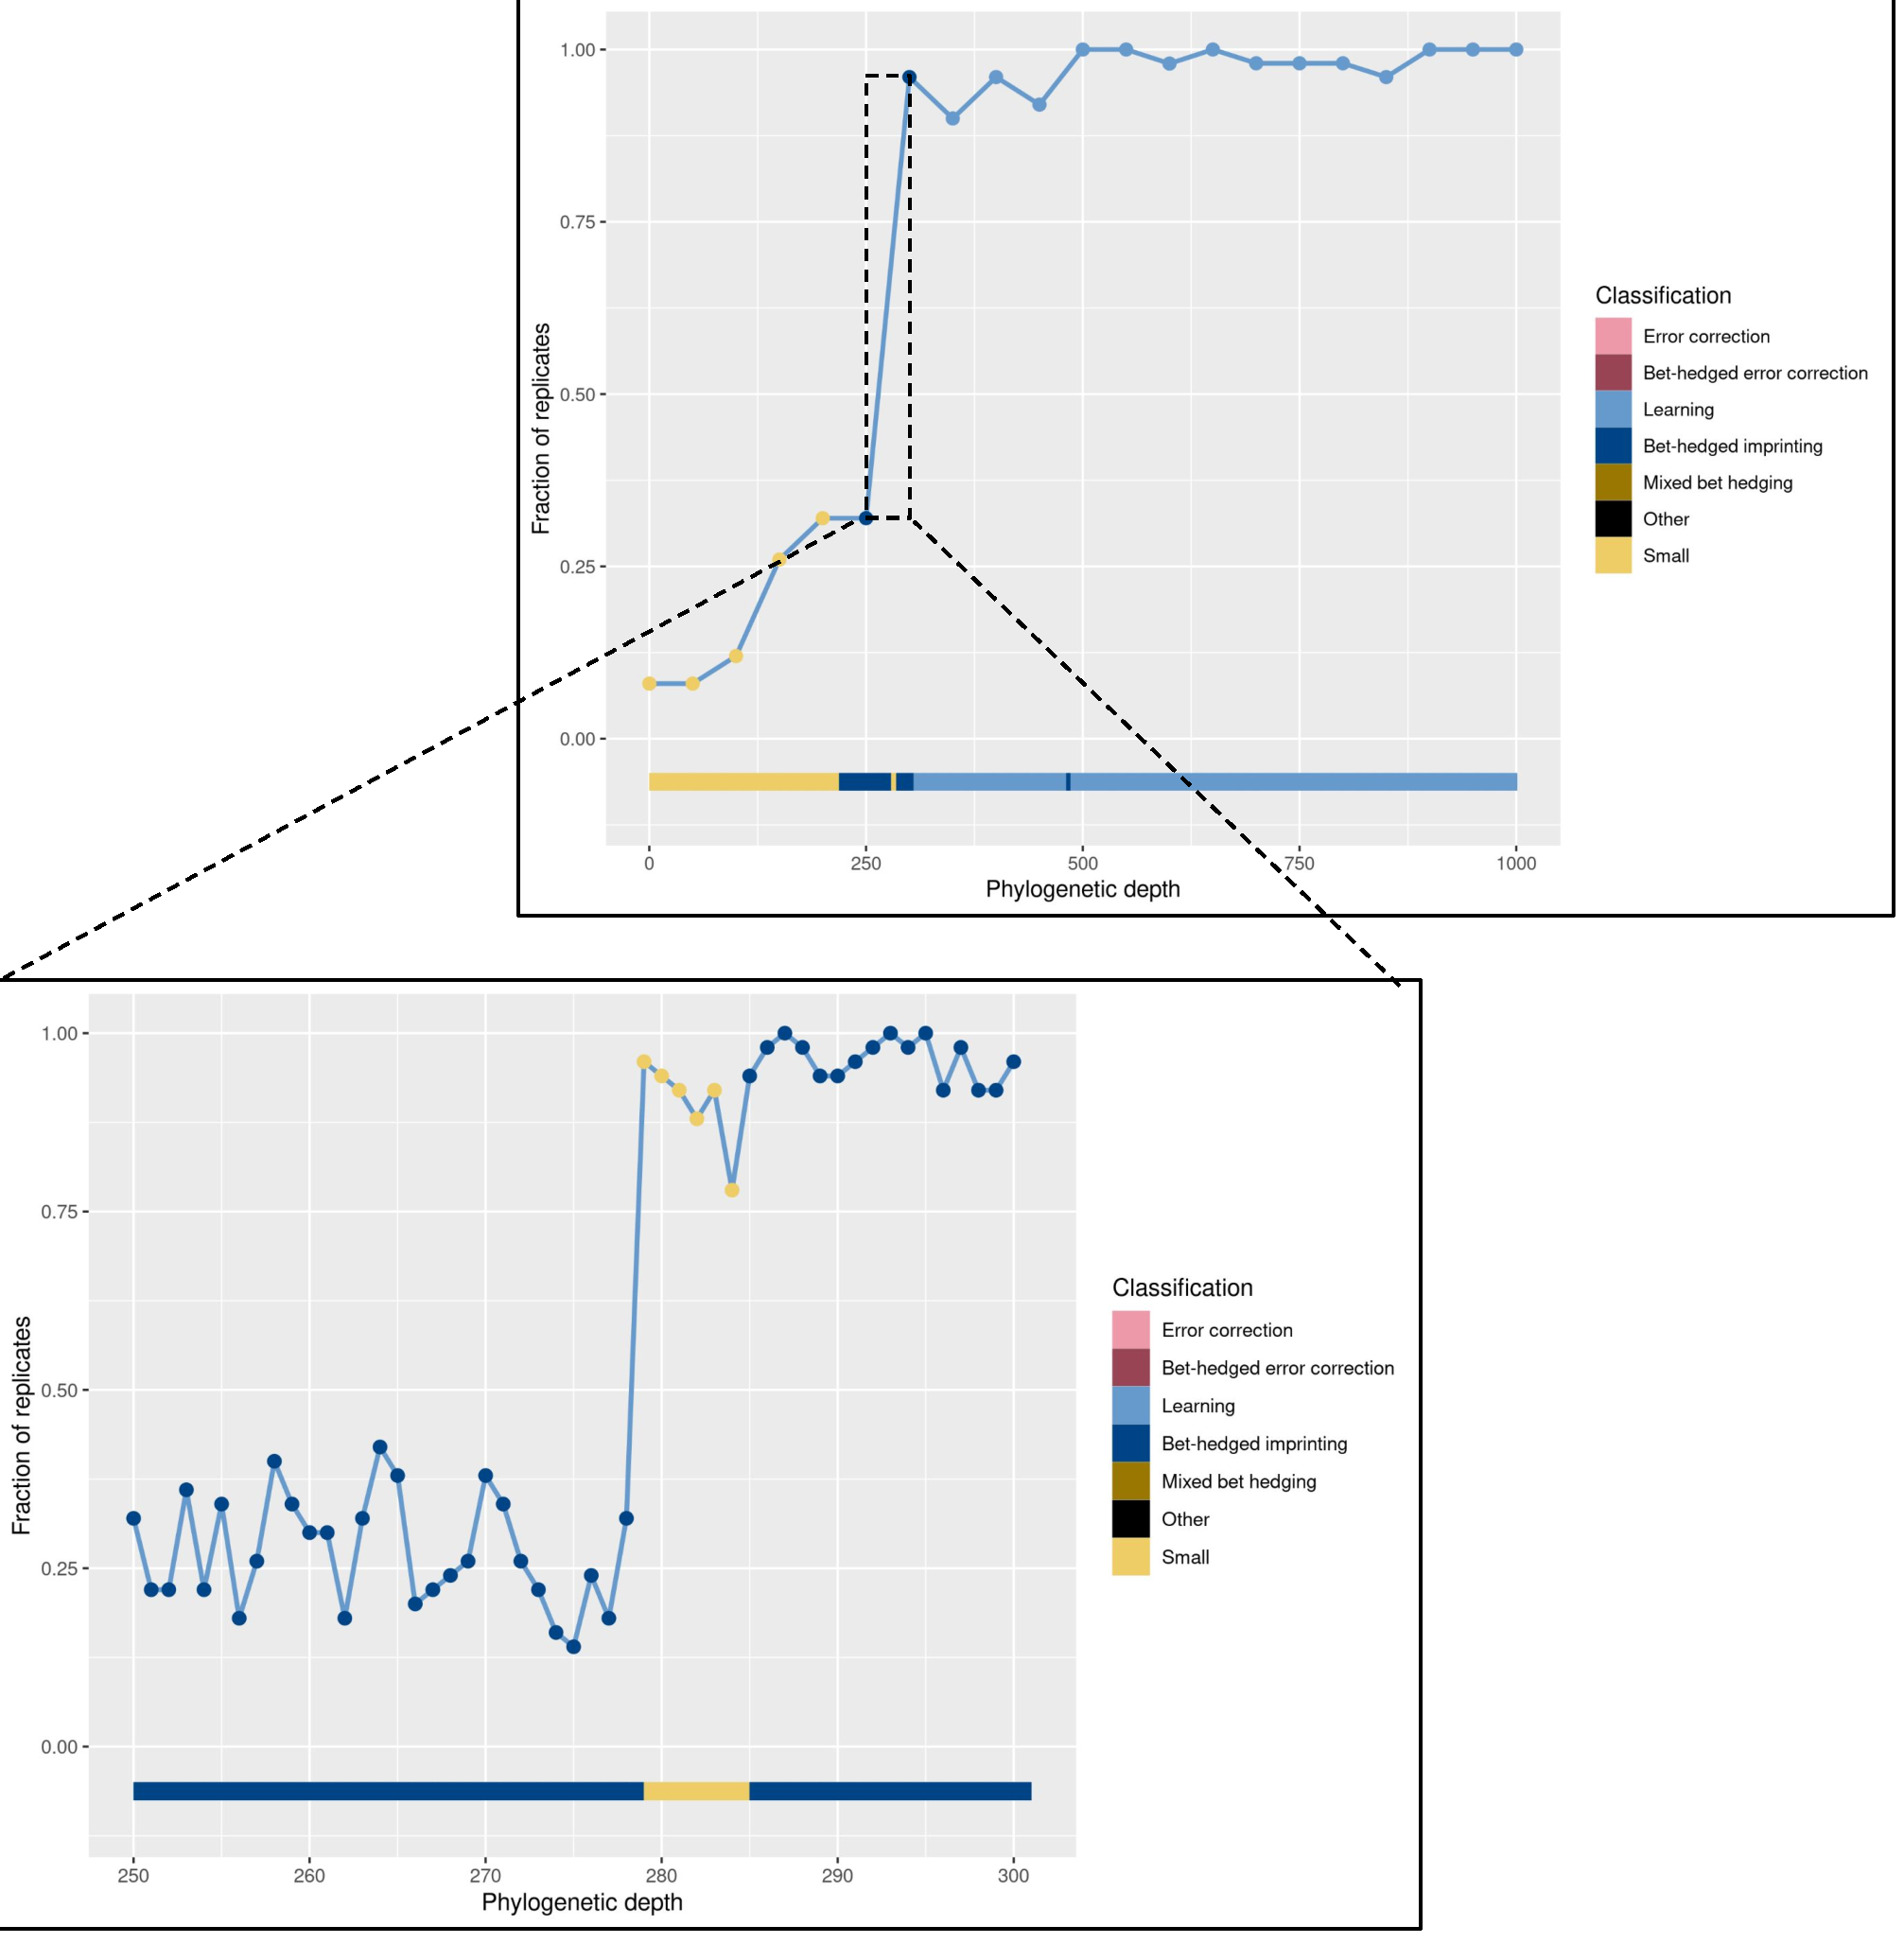
\includegraphics[width=0.45\textwidth]{media/test_pop_out_seed_15.pdf}
% \caption{
% \textbf{Case Study C}.
% Potentiation of associative learning as it changes over the lineage for Case Study C. 
% The top figure plot shows the results of the exploratory replays. 
% Two windows of increased potentiation were identified, indicated by the dashed rectangle. 
% Results of the targeted replays are shown in the bottom, pop-out plot.
% Both lines and points show potentiation at various steps along the lineage. 
% The color of the points corresponds to the behavior exhibited at that step of the lineage.
% The rectangle at the bottom of the plot also shows the behavior at the lineage, but with more detail than the evenly spaced points of the exploratory replay.}
% \label{fig-potentiation-case-study-d}
% \end{center}
% \end{figure}




\subsubsection{Lineage D}

% \begin{figure}[!h]
% \begin{center}
% 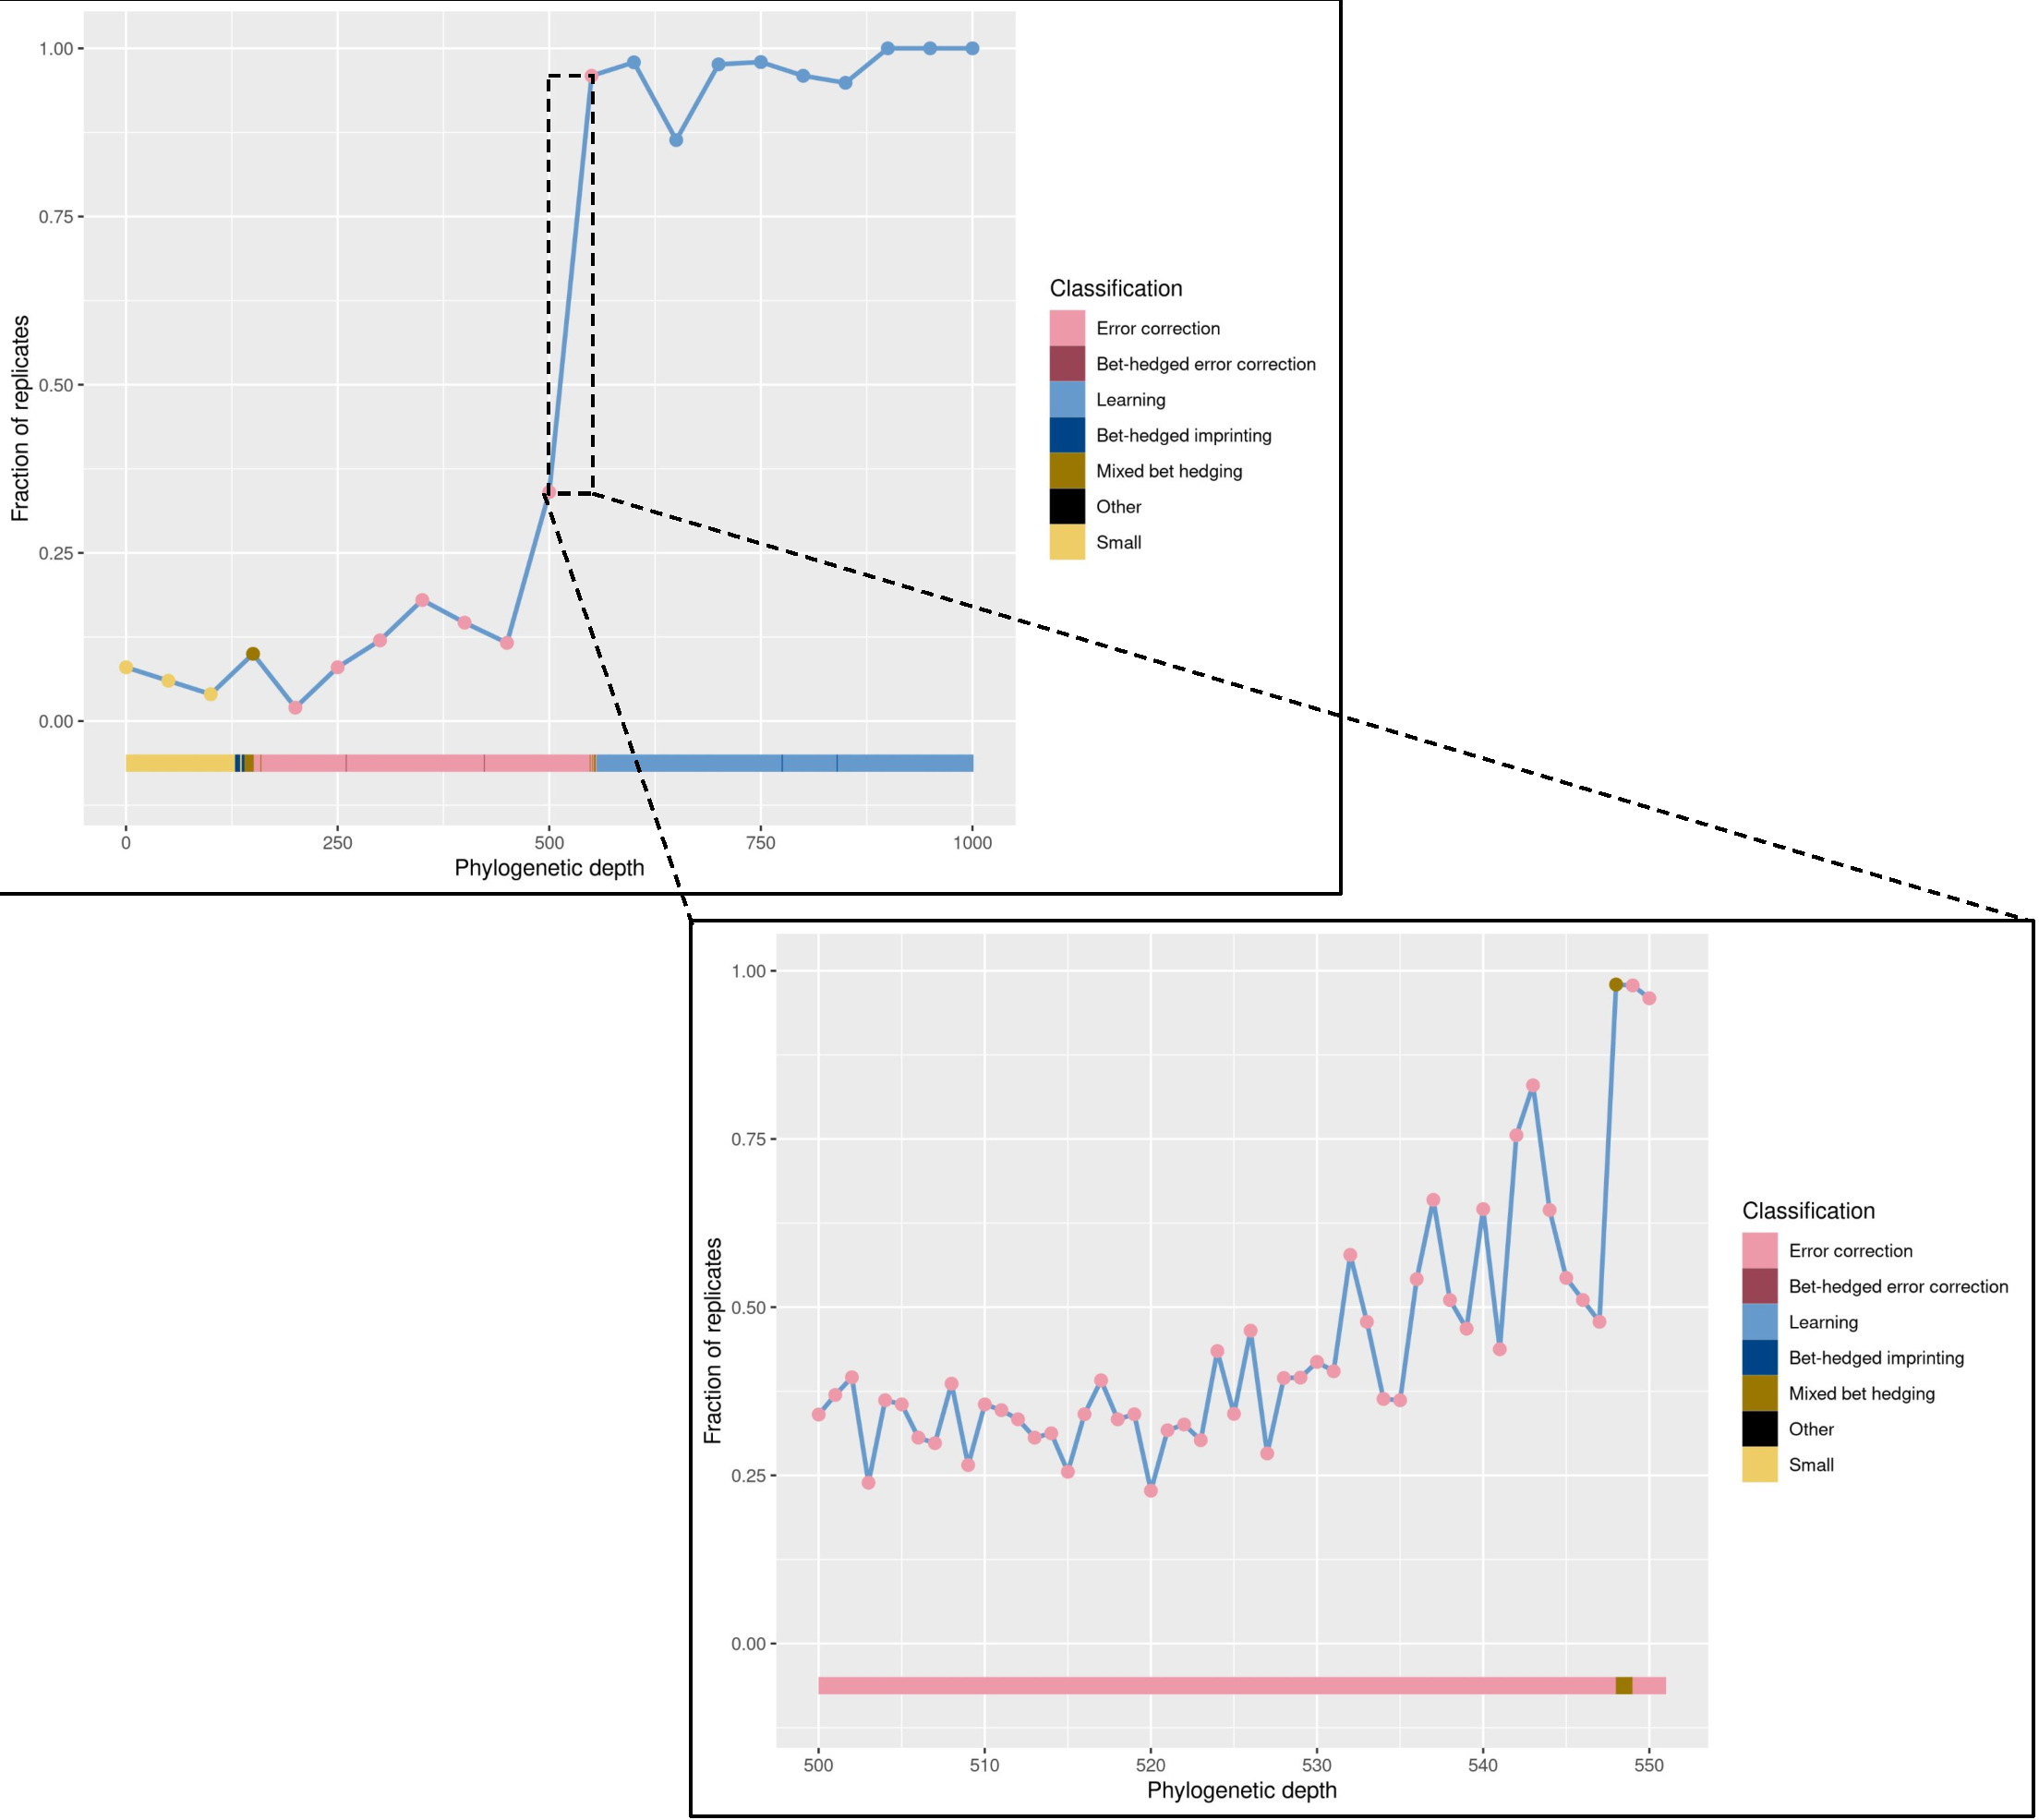
\includegraphics[width=0.45\textwidth]{media/test_pop_out_seed_6.pdf}
% \caption{
% \textbf{Case Study D}.
% Potentiation of associative learning as it changes over the lineage for Case Study D. 
% The top figure plot shows the results of the exploratory replays. 
% Two windows of increased potentiation were identified, indicated by the dashed rectangle. 
% Results of the targeted replays are shown in the bottom, pop-out plot.
% Both lines and points show potentiation at various steps along the lineage. 
% The color of the points corresponds to the behavior exhibited at that step of the lineage.
% The rectangle at the bottom of the plot also shows the behavior at the lineage, but with more detail than the evenly spaced points of the exploratory replay.}
% \label{fig-potentiation-case-study-d}
% \end{center}
% \end{figure}

Of the four replicates we analyzed, Lineage D is the only one that evolved error correction before learning.
Like the earlier lineages, the exploratory replays show that almost all potentiation comes from a single window. 
%Here, however, we only study the back half of the window, where 
In this case, potentiation grew from 34\% of replicates to 96\% between steps 500 and 550.
%Zooming in via targeted replays, potentiation in this window tells an interesting story. 
%It is hard to be certain given the noise of using 50 replay populations, but it appears that potentiation generally increases in the second half of the window. 
Targeted replays are especially noisy for this lineage, but generally show an increase in potentiation, especially in the latter half of the window.
%Of particular note are the last \~10 steps in this window. 
The largest jump in potentiation occurred at step 548, near the end of the window.
%Looking backward, however, other 
Prior mutations also showed notably increased potentiation, but in each case later mutations appeared to lower potentiation again. % before later mutations lowered it again. 
Specifically, steps 542 and 543 appear to have higher potentiation than the points around them, with potentiation dipping back below 50\% again before the largest jump at 548.

Out of all four lineages, D has the fewest steps between the largest potentiating step (548) and the first appearance of learning (556).
At the time, the potentiating mutations at 548 caused no discernible change in fitness even though they increased potentiation by 50 percentage points. 
Two mutations occurred at step 548: a point mutation swapped a flow control instruction for a math instruction and an insertion mutation added a comparative conditional instruction into the main execution loop. 
At step 548 the genotype encoded a naive error correction algorithm: after setup, organisms could always handle \textit{turn right} states, but always failed \textit{turn left} states, recovered, and then continued. 
%This changed when learning evolved 
At step 556, the algorithm started sensing the environment, albeit \textit{too} often. 
A mutation swapped a sensing instruction with a math instruction, and this combined with the prior comparison instruction from step 548 to allow the organism to move left when needed. 
The organism still blundered when it encountered a state sequence of \textit{left}, \textit{forward}, \textit{left}, but it quickly recovered. 
Since it can associate the cues with greater than 90\% accuracy, we classify it as learning. 
The local fitness landscape supports the idea that the comparison instruction was useful to the evolution of learning, as the potentiating mutation increased the number of learning genotypes in the two-step mutational neighborhood from under 800 to over 100,000.

% What's going on at 542/543?
Looking back at the apparent false start at steps 542 and 543, it is not clear what algorithmic changes these mutations conferred.
%, the potentiation mutations at steps 542 and 543 also altered 
These steps did, however, alter the set of learning behaviors that fell within the local mutational neighborhood. 
At step 541, there were only 324 two-step mutations that conferred learning, and only three of those resulted in a substantial fitness increase (a merit $> 10^{15}$). %; the merit of the best-performing mutant is ~$1.6e21$.
After steps 542 and 543, that number rose such that over 900 two-step mutations could confer learning, with over 500 resulting in a substantial fitness increase (including over 200 that reached a merit $> 10^{25}$.
We may be unsure of the exact effects of these mutations on the mechanics of the algorithm, but the changes in the local fitness landscape are profound. %to include learning algorithms with much higher fitness.
